\documentclass{standalone}
\usepackage{tikz,bm}
\begin{document}

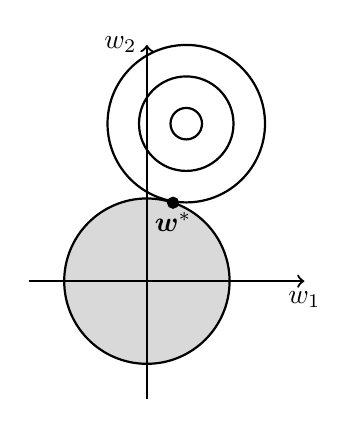
\begin{tikzpicture}

% Left Diagram
% Draw the origin
\coordinate (O) at (0.5, 2);

% Draw the contours (circles)
\draw[thick] (O) circle (0.2);
\draw[thick] (O) circle (0.6);
\draw[thick] (O) circle (1);
% \draw[thick] (O) circle (2.1);

% Draw the L2 ball (filled circle)
\filldraw[fill=gray!30, thick] (0,0) circle (1.05);

% Draw the optimal point
\filldraw[black] (1.05*0.316227766,1.05*0.9486832981) circle (2pt) node[anchor=north] {$\bm{w}^*$};

% Draw axes
\draw[thick,->] (-1.5,0) -- (2,0) node[anchor=north] {$w_1$};
\draw[thick,->] (0,-1.5) -- (0,3) node[anchor=east] {$w_2$};

\end{tikzpicture}

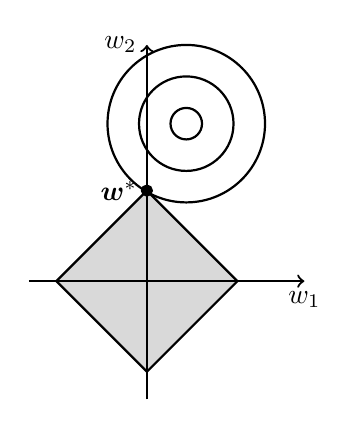
\begin{tikzpicture}

% Right Diagram
% Draw the origin
\coordinate (O) at (0.5, 2);

% Draw the contours (circles)
\draw[thick] (O) circle (0.2);
\draw[thick] (O) circle (0.6);
\draw[thick] (O) circle (1);
% \draw[thick] (O) circle (2.1);

% Draw the L1 ball (filled diamond)
\def\a{1.15}
\filldraw[fill=gray!30, thick] (-\a,0) -- (0,\a) -- (\a,0) -- (0,-\a) -- cycle;

% Draw the optimal point
\filldraw[black] (0,\a) circle (2pt) node[anchor=east] {$\bm{w}^*$};

% Draw axes
\draw[thick,->] (-1.5,0) -- (2,0) node[anchor=north] {$w_1$};
\draw[thick,->] (0,-1.5) -- (0,3) node[anchor=east] {$w_2$};

\end{tikzpicture}

\end{document}
